\section{Results}
\label{sec:results}

In this section, we present our findings based on implementing the gradient-free approach presented
earlier in Section~\ref{sec:method} for computing the active subspace, in~\ref{sub:cas}. 
The model output in the original space~($G$)
was approximated as $\mathcal{Y}$ in terms of active variables, $\vec\eta$ in the active subspace. A regression-fit
to $\mathcal{Y}$, $\tilde{\mathcal{Y}}$ was used as a surrogate for performing UQ. 
The accuracy of the surrogate was assessed by 
estimating the relative L-2 norm of the discrepancy between NEMD-based estimates and surrogate predictions,
and performing a comparative assessment in a probabilistic sense in~\ref{sub:ver}. The surrogate is further
used for estimating the total Sobol' indices which are shown to be consistent with the normalized activity scores,
evaluated using~\eqref{eq:ac} and~\eqref{eq:nac}, in~\ref{sub:gsa}.

\subsection{Computing the active subspace}
\label{sub:cas}

The iterative procedure outlined in Algorithm~\ref{alg:free} was used to compute the active subspace. 
We began
with an initial set of 5 samples in the 7-dimensional input space. The Monte Carlo samples were drawn
from the joint probability distribution of the uncertain SW parameters, considered
to be uniformly distributed in the interval $[0.9\theta_i^\ast,1.1\theta_i^\ast]$, where $\theta_i^\ast$ are the
nominal values provided in Table~\ref{tab:sw}. 
%
\begin{table}[htbp]
\centering
\ra{1.3}
\begin{tabular}{@{}ccccccc@{}}\toprule
$A$ & $B$ & $p$ & $q$ & $\alpha$ & $\lambda$ & $\gamma$ \\
7.05 & 0.60 & 4.0 & 0.0 & 1.80 & 21.0 & 1.20 \\
\bottomrule
\end{tabular}
\caption{Nominal values of the SW potential parameters~\cite{Stillinger:1985}.}
\label{tab:sw}
\end{table}
%
Initial set of model evaluations were used to estimate the gradient vector of thermal conductivity with
individual components representing the derivative with respect to $\xi_i$ corresponding to $\theta_i$ in
the physical space. At each iteration, $i$, model evaluations at 5 new samples in the full space were 
obtained and the quantity, $\vec{\varepsilon}^{(i)}$ was computed using~\eqref{eq:conv}.The iterative
procedure was terminated once the highest component of $\vec{\varepsilon}^{(i)}$ was found to be smaller than
the set tolerance, $\tau$ = 0.1. In this case, the process was observed to converge after 4 iterations
and required model evaluations at 25 samples, yielding $\max(\vec{\varepsilon}^{(i)})$~=~0.085.
 The resulting active subspace was found to be
1-dimensional. In Figure~\ref{fig:casfig1}, we plot the components of the dominant eigenvector (left),
and the quantity, $\max(\vec{\varepsilon}^{(i)})$, computed using components of the dominant eigenvector 
obtained between successive iterations, $i$ and $i-1$ (right) in~\eqref{eq:conv}.
%
\begin{figure}[htbp]
\begin{center}
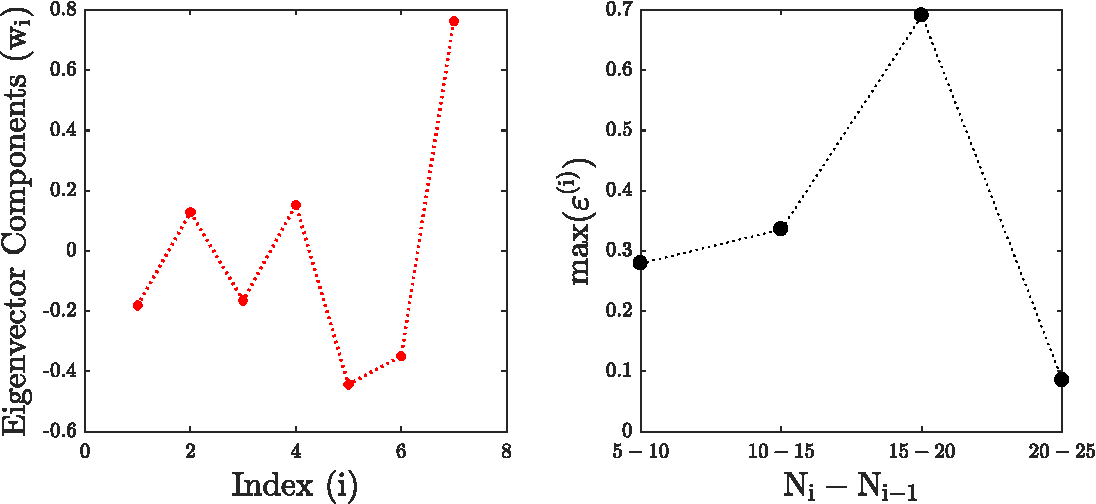
\includegraphics[width=0.8\textwidth]{./Figures/free_eigv5}
\caption{Left: Individual components of the dominant eigenvector that constitutes the 1-dimensional
active subspace. Right: A plot of $\max(\varepsilon^{(i)})$, obtained
using components of the dominant eigenvector between successive iterations.}
\label{fig:casfig1}
\end{center}
\end{figure}
%

The normalized eigenvalue spectrum is illustrated
in Figure~\ref{fig:casfig2}~(left), and the plot of $\mathcal{Y}$ vs. $\vec\eta$, regarded as the \textit{sufficient
summary plot} (SSP) is provided in Figure~\ref{fig:casfig2}~(right). 
%
\begin{figure}[htbp]
\begin{center}
\begin{tabular}{cc}
  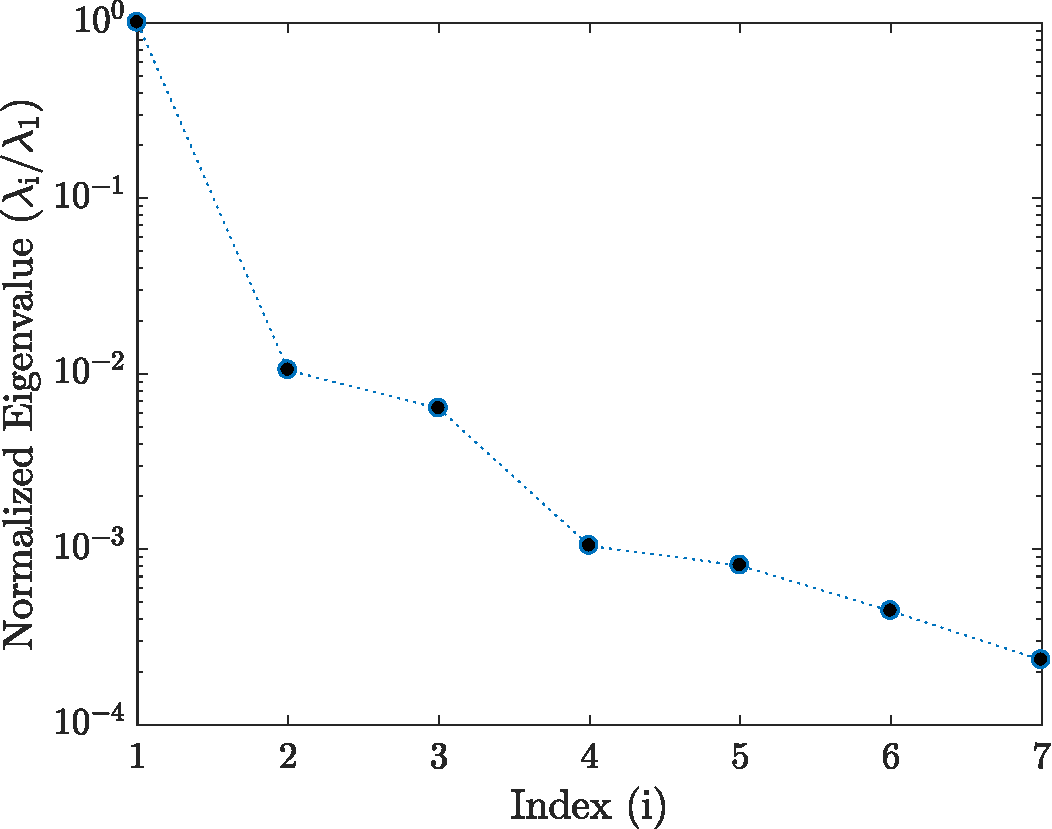
\includegraphics[width=0.42\textwidth]{./Figures/eig_spec}
  &
  \hspace{3mm}
  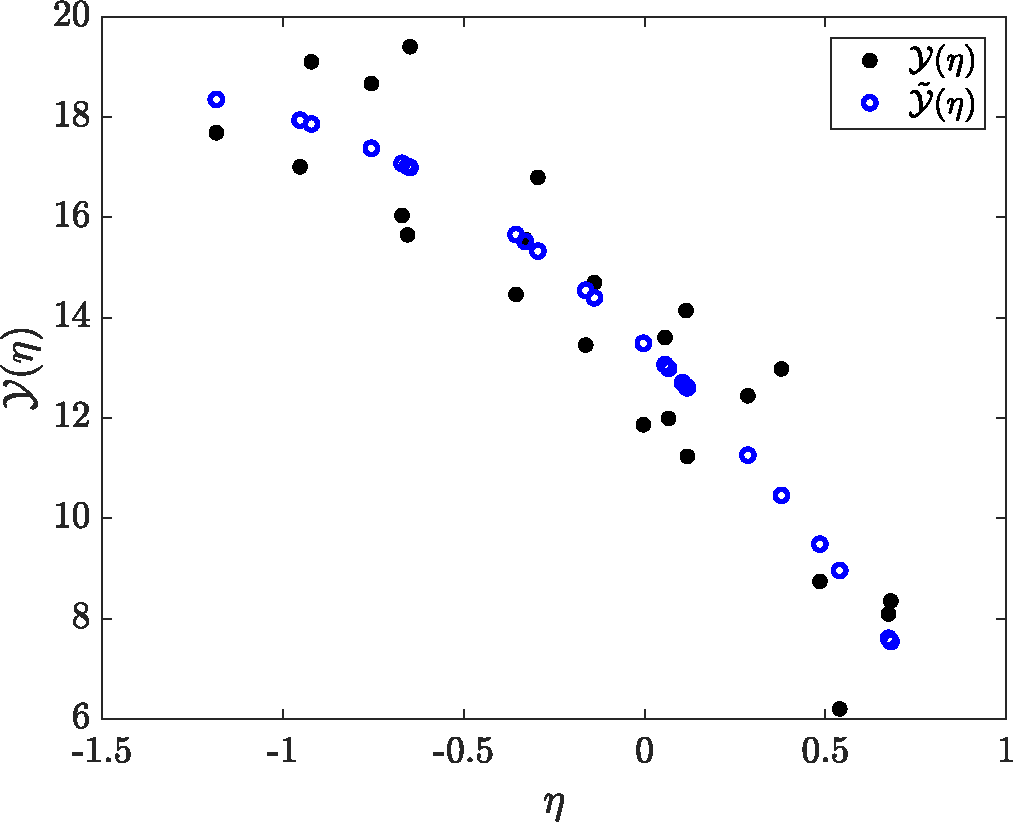
\includegraphics[width=0.4\textwidth]{./Figures/free_ssp1D}
  \end{tabular}
\caption{Left: Normalized eigenvalue spectrum of the converged matrix, $\hat{\mat{C}}$. Right: SSP
illustrating the variability of the NEMD-based thermal conductivity estimates in the 1-dimensional
active subspace.}
\label{fig:casfig2}
\end{center}
\end{figure}
%
Both plots confirm the existence of a 1-dimensional active subspace. The normalized eigenvalue spectrum
shows that the ratio of the first two eigenvalues, $\left(\frac{\lambda_1}{\lambda_2}\right)\sim\mathcal{O}(10^2)$.
Hence, the second largest eigenvalue is roughly two orders of magnitude smaller than the largest eigenvalue,
indicating a 1-dimensional subspace. Furthermore, the trends in the SSP seem to have been captured
reasonably well using a linear regression-fit which is also indicative of a 1-dimensional subspace. The linear 
fit is considered as a surrogate for $\mathcal{Y}$ i.e. $\tilde{\mathcal{Y}}$. In the following section, 
we verify the accuracy of the
surrogate. 


\subsection{Surrogate assessment}
\label{sub:ver}

The surrogate, $\tilde{\mathcal{Y}}$, illustrated in Figure~\ref{fig:casfig2}~(right) 
is assessed for accuracy at two levels: First, we perform a low-level assessment by estimating
 the relative L-2 norm of the difference
($\varepsilon_d$) between surrogate predictions and NEMD-based estimates of thermal conductivity 
of the Si bar in the active subspace ($\mathcal{Y}$) as follows:
%
\be
\varepsilon_d = \frac{\|\mathcal{Y}(\bm{\xi}) - \tilde{\mathcal{Y}}(\bm{\xi})\|_2}{\|\mathcal{Y}(\bm{\xi})\|_2}
\ee
%
The quantity, $\varepsilon_d$, was estimated to be roughly 0.1. In other words, the error introduced
due to approximating the function, $\mathcal{Y}$ by a surrogate, $\tilde{\mathcal{Y}}$ is about 10$\%$.
For many applications, this error might be too large, however, it is reasonable and
potentially acceptable for this problem considering that we are interested in approximating
the variability in thermal conductivity due to uncertainty in the SW
parameters. An exact UQ analysis in a 7-dimensional input space for an application involving
atomistic simulations would anyways be computationally impractical as discussed earlier in
Section~\ref{sec:intro}, and highlighted specifically in Table~\ref{tab:effort}.

Second, a higher level assessment of $\tilde{\mathcal{Y}}$ is performed wherein
the first-order and second-order 
statistics as well as probability distributions, obtained using the
surrogate and the set of available model evaluations at 35 samples in the 7-dimensional
input space are compared. Note that the surrogate predictions were obtained at the
same set of 35 samples for this purpose. Below, we provide a table consisting of the
mean and standard deviation of bulk thermal conductivity based on model and the
surrogate. Additionally, we plot a histogram based on model evaluations and compare
it with a probability density function (PDF), generated using kernel density estimation (KDE)
of surrogate predictions at 10$^5$ Monte Carlo samples in the 7-dimensional input domain. 
%
\begin{figure}[htbp]
\begin{center}
\begin{minipage}[htbp]{.25\linewidth}
\vspace{0pt}
%\centering
\hspace{-25mm}
\begin{tabular}{ccc}
\toprule
$\textbf{Distribution}$ & $\mu$ & $\sigma$ \\ 
\bottomrule
$G$~(Model) & 13.764 & 3.573 \\
$\tilde{\mathcal{Y}}$ (1D Surrogate) & 13.757 & 3.441 \\
\bottomrule
\end{tabular}
\end{minipage}
\hspace{5mm}
\begin{minipage}[htbp]{.25\linewidth}
\vspace{0pt}
%\centering
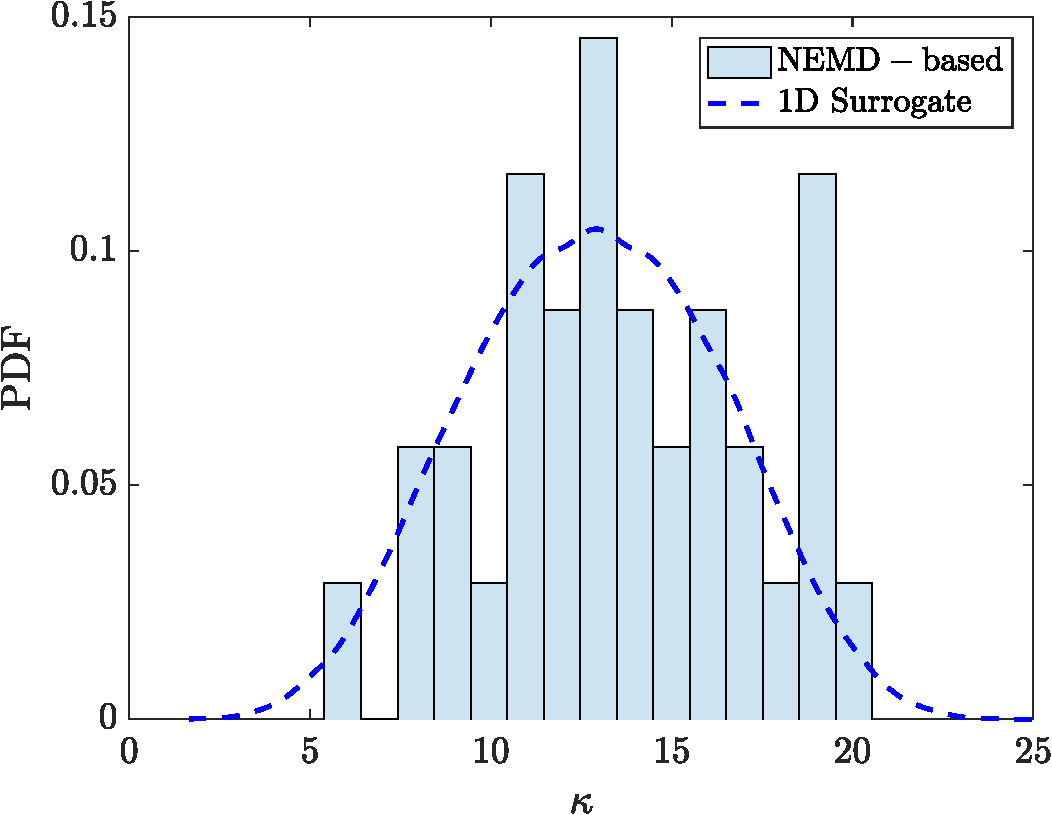
\includegraphics[width=3.0in]{./Figures/free_pdf_comp_SSP1D}
\end{minipage}%
\end{center} 
\caption{Left: Table providing the mean ($\mu$) and the standard deviation ($\sigma$) corresponding to
the model evaluations ($G$) and surrogate predictions ($\tilde{\mathcal{Y}}$)
at 35 samples in the cross-validation set. Right: A comparison of the histogram plot based on the
available set of 35 model evaluations and a PDF generated using surrogate predictions at 10$^5$
random samples in the 7-dimensional input domain.}  
\label{fig:level2}
\end{figure}
%
Both, first-order ($\mu$) and second-order ($\sigma$) statistics of the bulk thermal conductivity ($\kappa$),
obtained using the model and the surrogate are found to be in close agreement. Additionally, the
comparison of distributions in Figure~\ref{fig:level2} (right) confirms that the PDF captures the modal
estimate as well as the spread in $\kappa$ with reasonable accuracy. Hence, the surrogate based on
the 1-dimensional active subspace, evaluated earlier in~\ref{sub:cas} can be used to quantify and
characterize the uncertainty in bulk thermal conductivity of the Si bar due to the uncertainty in the
SW potential parameters. In the following section, we use the surrogate to estimate the total Sobol'
sensitivity indices of the SW parameters.  


\subsection{Global Sensitivity Analysis}
\label{sub:gsa}

Sobol total effect index, $\mathcal{T}(\theta_i)$, is one of the most commonly used variance-based 
measures for global
parametric sensitivity~\cite{Sobol:2001}. For a given input, $\theta_i$ and the corresponding output, 
$G(\theta_i)$, it accounts for the individual as well as coupled contributions of $\theta_i$ (due to
interaction with other inputs)
to the variability in the QoI. Mathematically, this is expressed as follows:
%
\be
\mathcal{T}(\theta_i) = 1 - 
\frac{\V[\mathbb{E}(G|\vec{\theta}_{\sim i})]}{\V(G)},
\label{eq:total}
\ee
%
where $\vec{\theta}_{\sim i}$ is a vector of all but the $i^{th}$ input. Note that the framework for 
estimating $\mathcal{T}(\theta_i)$ assumes that the individual inputs are statistically independent.
Several extensions have been proposed for GSA in situations involving a correlated set of
inputs~\cite{Borgonovo:2007,Li:2010,Jacques:2006,Xu:2007,Hart:2017}. However, in the present work,
the SW parameters are considered to be independent. 

A pertinent challenge associated with  the computation of $\mathcal{T}(\theta_i)$ is the associated
computational effort considering tens of thousands of model evaluations are typically needed to obtained
converged estimates. Hence, for the present application, GSA would be intractable. However, we mitigate
this challenge by estimating $\mathcal{T}(\theta_i)$ using predictions of the surrogate model, 
$\tilde{\mathcal{Y}}$ at a large set of pseudorandom samples in the 7-dimensional physical domain.  
Moreover, as discussed earlier in Section~\ref{sec:method}, components of the eigenvectors in the
active subspace could be used for estimating the activity scores (see~\eqref{eq:ac}) for the purpose of GSA.
A bar-graph illustrating the normalized activity scores of the SW potential parameters is illustrated in
Figure~\ref{fig:gsa}. Additionally, we have included estimates of $\mathcal{T}(\theta_i)$, computed using
the 1-dimensional surrogate. 
%
\begin{figure}[htbp]
\begin{center}
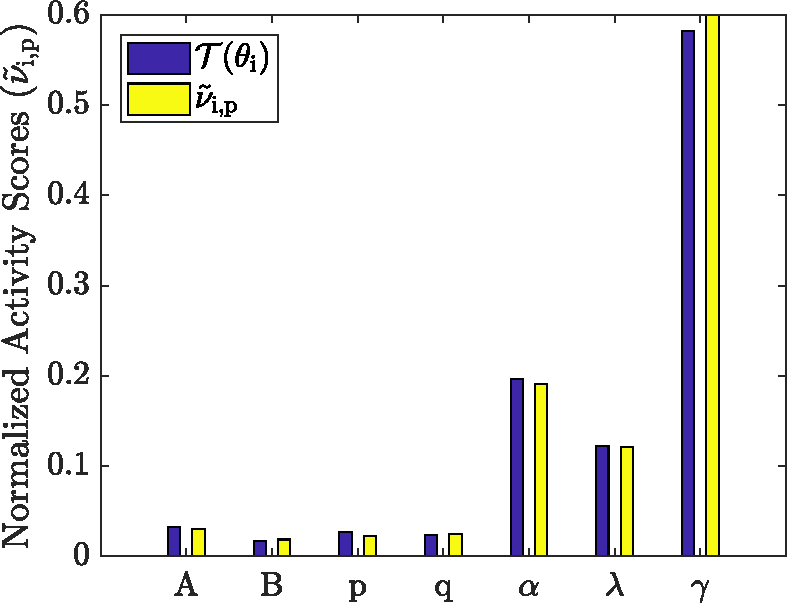
\includegraphics[width=0.45\textwidth]{./Figures/free_as_gsa}
\caption{A comparative assessment of the Sobol total-effect index, $\mathcal{T}(\theta_i)$, and the normalized
activity scores, $\tilde{\nu}_{i,p}$, for GSA of the SW potential parameters.}
\label{fig:gsa}
\end{center}
\end{figure}
%
The sensitivity estimates based on the two approaches are found to be consistent. This is expected since
both, the surrogate and the dominant eigenvectors are associated with the active subspace. Moreover, it
was shown in~\cite{Vohra:2018c} that the activity scores can be used to approximate the bounds on Sobol
total-effect indices. The above result indicates that the variability in bulk thermal conductivity is predominantly
due to the uncertainty in $\alpha$, $\lambda$, and $\gamma$. This is also consistent with our earlier
findings involving GSA using DGSMs~\cite{Vohra:2018b}~(see Figure~7 therein). While we have focused on uncertainty
propagation in this work, this result could be exploited to reduce computational effort associated with
calibration of the SW parameters. Specifically, it seems pragmatic to allocate bulk of the computational
resources for calibrating the important parameters: $\alpha$, $\lambda$, and $\gamma$.  
